% Clase del documento
\documentclass[12pt,twoside,titlepage]{report}





%%%%%%%%%%%%%%%%%%%%%%% Paquetes %%%%%%%%%%%%%%%%%%%%%%%

\usepackage[a4paper,bindingoffset=3mm,bottom=35mm]{geometry}


% Usad \usepackage[dvips]{graphicx} o \usepackage[pdftex]{graphicx} (no ambos)
%\usepackage[dvips]{graphicx} %%% para LaTeX. Las figuras deben estar en formato eps

\usepackage[colorlinks=true,pdftex]{hyperref}   %%% Opcional. Para incluir marcadores y enlaces en el pdf
\usepackage[pdftex]{graphicx}  %%% para pdflatex. Las figuras pueden estar en pdf, jpg, svg y otros formatos


\usepackage[spanish]{babel}

%\usepackage[latin1]{inputenc} % Usad en WinEdt/MikTex
\usepackage[utf8]{inputenc} % Usad en overleaf

%\usepackage[T1]{fontenc}


% Algunos paquetes útiles

\usepackage{amsmath,amssymb}
\usepackage{hyperref}
\usepackage{color}
\usepackage{afterpage}
\usepackage{paralist}
\usepackage{array}
\usepackage{enumerate}
\usepackage{paralist}
\usepackage{enumitem}
\usepackage{float}
\usepackage{setspace}
\usepackage{listings}
\usepackage{algorithm}
\usepackage{algorithmic}
\usepackage{fancyhdr}
\usepackage{rotating}
\usepackage{multirow}


% Otros paquetes

\usepackage{quotchap}
\usepackage{lipsum}

%%%%%%%%%%%%%%%%%%%%%%%%%%%%%%%%%%%%%%%%%%%%%%%%%%%%%%%%






%%%%%%%%%%%%%%%%%%%%%%% Definiciones básicas %%%%%%%%%%%%%%%%%%%%%%%

\newcommand{\nombreautor}{Oscar Nydza Nicpoñ}
\newcommand{\nombretutor}{Juan Manuel Serrano Hidalgo}
\newcommand{\titulotrabajo}{Comparativa entre las API de Spark en Scala y Python}
\newcommand{\escuela}{Escuela Técnica Superior\\de Ingeniería Informática}
\newcommand{\escuelalargo}{Escuela Técnica Superior de Ingeniería Informática}
\newcommand{\universidad}{Universidad Rey Juan Carlos}
\newcommand{\fecha}{Fecha}
\newcommand{\grado}{Grado en Ingeniería de Computadores}
\newcommand{\curso}{Curso 2021-2022}
\newcommand{\logoUniversidad}{logoURJC.pdf} % logoURJC.eps

%%%%%%%%%%%%%%%%%%%%%%%%%%%%%%%%%%%%%%%%%%%%%%%%%%%%%%%%%%%%%%%%%%%%






%%%%%%%%%%%%%%%%%%%%%%%%% Otras definiciones %%%%%%%%%%%%%%%%%%%%%%%%%%

% Definiciones de colores (para hidelinks)
\definecolor{BlueLink}{rgb}{0.165,0.322,0.745}
\definecolor{PinkLink}{rgb}{0.8,0.22,0.5}
\definecolor{gray}{rgb}{0.6,0.6,0.6}


% Enlaces
\hypersetup{hidelinks,pageanchor=true,colorlinks,citecolor=PinkLink,urlcolor=black,linkcolor=BlueLink}


\newcommand\blankpage{%
    \newpage
    \null
    \thispagestyle{empty}%
    %\addtocounter{page}{-1}%
    \newpage}


% Texto referencias
\addto{\captionsspanish}{\renewcommand{\bibname}{Bibliografía}}

% Texto Índice de tablas
\addto\captionsspanish{
\def\tablename{Tabla}
\def\listtablename{\'{I}ndice de tablas}
}


\floatname{algorithm}{Algoritmo}

\newfloat{algorithm}{t}{lop}


%\newenvironment{pseudocodigo}[1][htb]
%  {\renewcommand{\algorithmcfname}{Pseudocódig}% Update algorithm name
%   \begin{algorithm}[#1]%
%  }{\end{algorithm}}
  
%%%%%%%%%%%%%%%%%%%%%%%%%%%%%%%%%%%%%%%%%%%%%%%%%%%%%%%%%%%%%%%%%%%%





%%%%%%%%%%%%%%%%%%%%%%% Estilo de código (en Python) %%%%%%%%%%%%%%%%%%%%%%%

\definecolor{bg}{rgb}{0.95,0.95,0.95}
\definecolor{mydeepteal}{rgb}{0.16,0.22,0.23}
\definecolor{myteal}{rgb}{0.31,0.44,0.46}
\definecolor{mymediumteal}{rgb}{0.41,0.58,0.60}

\DeclareFixedFont{\ttb}{T1}{txtt}{bx}{n}{12} % for bold
\DeclareFixedFont{\ttm}{T1}{txtt}{m}{n}{12}  % for normal


%\newcommand*{\FormatDigit}[1]{\textcolor{mydeepteal}{#1}}
\newcommand*{\FormatDigit}[1]{\textcolor{black}{#1}}

% Python style for highlighting
\newcommand\mypythonstyle{\lstset{
language=Python,
basicstyle=\ttfamily\small,
%basicstyle=\linespread{1.0}\footnotesize\ttm,
otherkeywords={self},             % Add keywords here
keywordstyle=\bfseries\ttfamily\color{myteal},
%keywordstyle=\ttb\color{myteal},
commentstyle=\itshape\color{myteal},
stringstyle=\color{mydeepteal},
emph={MyClass,__init__},          % Custom highlighting
emphstyle=\ttb\color{mydeepteal},    % Custom highlighting style
% Any extra options here
showstringspaces=false,            %
backgroundcolor=\color{bg},
rulecolor = \color{bg},
%identifierstyle=\color{deepgreen},
breaklines=true,
numbers=left,
numbersep=5pt,
numberstyle=\tiny,
tabsize=4,
xleftmargin=1em,
frame = single,
framesep = 3pt,
framextopmargin=0pt,
framexbottommargin=0pt,
framexleftmargin=0pt,
framexrightmargin=0pt,
fontadjust=true,
basewidth=0.55em, % compactness of code
upquote=true,
}}

% Python environment
\lstnewenvironment{mypython}[1][]
{
\mypythonstyle
\lstset{#1}
}
{}

\newcommand\mypythonstylenormalinline{\lstset{
language=Python,
basicstyle=\ttfamily\normalsize,
%basicstyle=\linespread{1.0}\footnotesize\ttm,
otherkeywords={self},            % Add keywords here
keywordstyle=\bfseries\ttfamily\color{myteal},
%keywordstyle=\ttb\color{myteal},
commentstyle=\itshape\color{mymediumteal},
stringstyle=\color{mydeepteal},
emph={MyClass,__init__},          % Custom highlighting
emphstyle=\ttb\color{mydeepteal},    % Custom highlighting style
% Any extra options here
showstringspaces=false,            %
backgroundcolor=\color{bg},
rulecolor = \color{bg},
%identifierstyle=\color{deepgreen},
breaklines=false,
numbers=left,
numbersep=5pt,
numberstyle=\tiny,
tabsize=4,
xleftmargin=0em,
frame = single,
framesep = 3pt,
framextopmargin=0pt,
framexbottommargin=0pt,
framexleftmargin=0pt,
framexrightmargin=0pt,
fontadjust=true,
%basewidth=0.55em, % compactness of code
upquote=true,
}}

\newcommand\mypythoninline[1]{{\mypythonstylenormalinline\lstinline!#1!}}

%%%%%%%%%%%%%%%%%%%%%%%%%%%%%%%%%%%%%%%%%%%%%%%%%%%%%%%%%%%%%%%%%%%%%%%%%%%%%%

\usepackage{listings}

% "define" Scala
\lstdefinelanguage{scala}{
  morekeywords={abstract,case,catch,class,def,%
    do,else,extends,false,final,finally,%
    for,if,implicit,import,match,mixin,%
    new,null,object,override,package,%
    private,protected,requires,return,sealed,%
    super,this,throw,trait,true,try,%
    type,val,var,while,with,yield},
  otherkeywords={=>,<-,<\%,<:,>:,\#,@},
  sensitive=true,
  morecomment=[l]{//},
  morecomment=[n]{/*}{*/},
  morestring=[b]",
  morestring=[b]',
  morestring=[b]"""
}

\usepackage{color}
\definecolor{dkgreen}{rgb}{0,0.6,0}
\definecolor{gray}{rgb}{0.5,0.5,0.5}
\definecolor{mauve}{rgb}{0.58,0,0.82}

\lstset{frame=tb,
  language=scala,
  aboveskip=3mm,
  belowskip=3mm,
  showstringspaces=false,
  columns=flexible,
  basicstyle={\small\ttfamily},
  numbers=none,
  numberstyle=\tiny\color{gray},
  keywordstyle=\color{blue},
  commentstyle=\color{dkgreen},
  stringstyle=\color{mauve},
  frame=single,
  breaklines=true,
  breakatwhitespace=true
  tabsize=3
}


%%%%%%%%%%%%%%%%%%%%%%%%%%%% Comandos definidos por el autor 

\newcommand{\transpuesta}{\mbox{\tiny $\mathsf{T}$}}








%%%%%%%%%%%%%%%%%%%%%%%%%%%%%%%%%%%%%%%%%%%%%%%%%%%%%%%%%%%%%%%%%%%%%%%
%                           Inicio del documento                       
%%%%%%%%%%%%%%%%%%%%%%%%%%%%%%%%%%%%%%%%%%%%%%%%%%%%%%%%%%%%%%%%%%%%%%%


\begin{document}

\pagestyle{plain}




%%%%%%%%%%%%%%%%%%%%%%%%%%%%%%%%%%%% Portada %%%%%%%%%%%%%%%%%%%%%%%%%%%%%%%%%%

%\pagenumbering{gobble}
%\pagenumbering{arabic}

% Universidad, Facultad
\begin{titlepage}
\selectlanguage{spanish}


% logo
\begin{center}
    \includegraphics[scale=0.7]{\logoUniversidad}
\end{center}

\bigskip

\begin{center}
\begin{LARGE}
\escuela \\
\end{LARGE}
\end{center}

\bigskip
\bigskip

% Grado
\begin{center}
\begin{large}
\textbf{\grado}\\
\end{large}
\end{center}

% Curso
\begin{center}
\begin{large}
\textbf{\curso}\\
\end{large}
\end{center}

\bigskip

\textbf{\begin{center}
\begin{large}
\textbf{Trabajo Fin de Grado}
\end{large}
\end{center}}

\bigskip
\bigskip
\bigskip

% Nombre del TFG
\begin{center}
\textbf{\begin{large}
\MakeUppercase{\titulotrabajo}\\
\end{large}}
\end{center}

% Nombre del autor
\vspace{\fill}
\begin{center}
\textbf{Autor: \nombreautor}\\ \smallskip
% Tutor
\textbf{Tutor: \nombretutor}\\
% Añadir segundo tutor si hubiera


\bigskip

% Fecha
%\textbf{\fecha}\\
\end{center}
\end{titlepage}


%%%%%%%%%%%%%%%%%%%%%%%% Opcional %%%%%%%%%%%%%%%%%%%%%%
%\blankpage

%\thispagestyle{empty}
%\begin{center}

% Nombre del trabajo
%\textbf{\begin{large}
%\MakeUppercase{\titulotrabajo}\\*
%\end{large}}
%\vspace*{0.2cm}
%\vspace{5cm}

% Nombre del autor y del tutor
%\large Autor: \nombreautor \\* \medskip
%\large Tutor: \nombretutor \\*

%\vfill

% Escuela, universidad y fecha
%\escuelalargo \\ \smallskip
%\universidad \\
%\vspace{1cm}
%\fecha \\

%\clearpage

%\end{center}
%%%%%%%%%%%%%%%%%%%%%%%%%%%%%%%%%%%%%%%%%%%%%%%%%%%%%%%%

\hypersetup{pageanchor=true}

\normalsize
\afterpage{\blankpage} % Se deben añadir página en blanco para que lo capítulos de la memoria o estas secciones introductorias empiecen en páginas impares

%%%%%%%%%%%%%%%%%%%%%%%%%%%%%%%%%%%%%%%%%%%%%%%%%%%%%%%%%%%%%%%%%%%%%%%%%%%%%%%





% Estilo de párrafo de los capítulos
\setlength{\parskip}{0.75em}
\renewcommand{\baselinestretch}{1.25}
% Interlineado simple
\spacing{1}

\pagenumbering{Roman}
\setcounter{page}{2}


%%%%%%%%%%%%%%%%%%%%%%%%% Agradecimientos o dedicatoria %%%%%%%%%%%%%%%%%%%%%%%%%%%

\chapter*{Agradecimientos}

Breves agradecimientos o dedicatoria.

\afterpage{\blankpage}

%%%%%%%%%%%%%%%%%%%%%%%%%%%%%%%%%%%%%%%%%%%%%%%%%%%%%%%%%%%%%%%%%%%%%%%%%%%%%%%%%%%






%%%%%%%%%%%%%%%%%%%%%%%%%%%%%%%%%%%% Resumen %%%%%%%%%%%%%%%%%%%%%%%%%%%%%%%%%%%%%%

\chapter*{Resumen}

Breve resumen del Trabajo de Fin de Grado (TFG). Recomendable entre 250-300 palabras, conteniendo los principales objetivos y resultados derivados del mismo.

\mbox{} \bigskip

\noindent \textbf{Palabras clave}:
\begin{compactitem}
    \item Python
    \item Ciberseguridad
    \item Aprendizaje automático (pueden ser varias)
    \item $\ldots$
\end{compactitem}

\afterpage{\blankpage}

%%%%%%%%%%%%%%%%%%%%%%%%%%%%%%%%%%%%%%%%%%%%%%%%%%%%%%%%%%%%%%%%%%%%%%%%%%%%%%%%%%%





%%%%%%%%%%%%%%%%%%%%%%%%%%%%%%%%%%%% Índices %%%%%%%%%%%%%%%%%%%%%%%%%%%%%%%%%%%%

% Estilo de párrafo de los Índices
\setlength{\parskip}{1pt}
\renewcommand{\baselinestretch}{1}
\renewcommand{\contentsname}{Índice de contenidos}


% Índice de contenidos
\tableofcontents
\afterpage{\blankpage}

% Índice de tablas (OPCIONAL)
%\listoftables
%\afterpage{\blankpage}
%\addcontentsline{toc}{chapter}{\noindent \listtablename}

% Índice de figuras (OPCIONAL)
\listoffigures
\afterpage{\blankpage}
\addcontentsline{toc}{chapter}{\listfigurename}

% Índice de códigos/algoritmos (OPCIONAL).   El término "Códigos" se puede cambiar por "Métodos", "Funciones", "Algoritmos", etc.
\renewcommand\lstlistlistingname{Códigos}
\renewcommand\lstlistingname{Código}
\renewcommand\lstlistlistingname{Índice de códigos}

\lstlistoflistings
\afterpage{\blankpage}
\addcontentsline{toc}{chapter}{\lstlistlistingname}


% En este documento (de momento) no se ha considerado incluir un índice de algoritmos/pseudocódigos, como el que aparece en \ref{AdditionalLouvain}

%%%%%%%%%%%%%%%%%%%%%%%%%%%%%%%%%%%%%%%%%%%%%%%%%%%%%%%%%%%%%%%%%%%%%%%%%%%%%%%%%%%





%%%%%%%%%%%%%%%%%%%%%%% Cabeceras y pies de página (Opcional) %%%%%%%%%%%%%%%%%%%%%%%

%\setlength{\headheight}{15.2pt}
\pagestyle{fancy}


\renewcommand{\chaptermark}[1]{\markboth{Capítulo \thechapter.\ #1}{}}

\pagestyle{fancy}
\fancyhf{}
\fancyhead[LO]{\leftmark}
\fancyhead[RO]{}
\fancyhead[RE]{\nouppercase\rightmark}
\fancyhead[LE]{}
\fancyfoot[C]{\thepage}

%%%%%%%%%%%%%%%%%%%%%%%%%%%%%%%%%%%%%%%%%%%%%%%%%%%%%%%%%%%%%%%%%%%%%%%%%%%%%%%%%%%%






%%%%%%%%%%%%%%%%%%%%%%%%%%%%%% Capítulos de la memoria %%%%%%%%%%%%%%%%%%%%%%%%%%%%%



% Capítulo 1
\chapter{Introducción}
\newpage

%%%%%%%%%%%%%%%%%%%%%%%%%%%%%%%%%%%%%%%%%%%%%%%%%%%%%%%%%%%%%%%%%%%%%%%%%%

% Estilo resto de páginas
\pagestyle{fancy}


% Estilo de párrafo de los capítulos
\setlength{\parskip}{0.75em}
\renewcommand{\baselinestretch}{1.25}
% Interlineado simple
\spacing{1}
% Numeración contenido
\pagenumbering{arabic}
\setcounter{page}{1}

%%%%%%%%%%%%%%%%%%%%%%%%%%%%%%%%%%%%%%%%%%%%%%%%%%%%%%%%%%%%%%%%%%%%%%%%%%



Se puede añadir texto antes de empezar la primera sección.


\section{Contexto y alcance}

Contexto. Situar al lector. Objetivo general y alcance del trabajo.


\section{Estructura del documento}

La estructura del TFG no es fija. El tutor indicará una estructura adecuada dependiendo del trabajo concreto.

Se puede incluir dentro de cada apartado secciones adicionales. La copia en papel de la memoria del TFG será encuadernada en pasta dura de color azul (p.e. encuadernación tipo chanel). La portada, que puede ser una pegatina transparente, seguirá el modelo que se adjunta, que incluye el escudo y nombre de la URJC, la titulación cursada por el alumno, el curso académico, el título del TFG, el autor y el o los directores/tutores.


\subsection{Trabajos de grados en informática}

Una posible estructura de la memoria final asociada con cada TFG podría ser la siguiente (leed la normativa de TFG):
\begin{enumerate}
 \item Introducción
 \item Objetivos (incluyendo descripción del problema, estudio de alternativas y metodología empleada)
 \item Descripción informática (puede incluir especificación, diseño, implementación y pruebas).
 \item Experimentos / validación
 \item Conclusiones (incluyendo los logros principales alcanzados y posibles trabajos futuros)
 \item Bibliografía
 \item Apéndices
\end{enumerate}


\subsection{Trabajos del grado en matemáticas}

Una posible estructura de la memoria final asociada con cada TFG podría ser la siguiente:
\begin{enumerate}
 \item Introducción
 \item Objetivos (incluyendo descripción del problema, estudio de alternativas y metodología empleada)
 \item Material y métodos / Metodología / Cuerpo del trabajo (describir las metodologías empleadas en el desarrollo del TFG o el desarrollo del mismo en caso de ser un trabajo de recopilación bibliográfica sobre un tema).
 \item Resultados (opcional, dependiendo del tipo de trabajo desarrollado)
 \item Conclusiones (incluyendo los logros principales alcanzados y posibles trabajos futuros)
 \item Bibliografía
 \item Apéndices
\end{enumerate}


% \afterpage{\blankpage} % puede generar problema en índice de contenidos
% \newpage







% Capítulo 2
\chapter{Objetivos}
\newpage

El principal objetivo de este Trabajo de Fin de Grado realizar una comparativa entre las API de Spark de Scala y de Python. Sin embargo, también existen otros objetivos que irán surgiendo mientras se avanza sobre el principal. Entre ellos estarían:

\begin{enumerate}
  \item Aprender Scala como lenguaje funcional: para ello utilizaré distintos recursos bibliográficos, pero principalmente "Programming In Scala", 4ª edición, de Martin Odersky y "Functional Programming in Scala" 1ª edición, de Paul Chiusano. Se aprenderán conceptos como las funciones de orden superior, tipos de datos algebráicos, currificación de funciones y recursividado la correspondencia de Curry-Howard.
  \item Aprender Spark como API tanto para Scala como para Python: para ello principalmente usaré el libro "Spark: The Definitive Guide", de Bill Chambers. Aprenderé conceptos como la API de DataFrames, Spark SQL en profundidad cómo utilizar la Spark UI para obtener métricas del proceso.
  \item Visualizar de los resultados de las queries realizadas usando Plotly. 
  \item Migrar queries desde PySpark a Scala Spark, centrando la explicación en las diferencias entre ambas APIs y en detalles a tener en cuenta al hacer una migración de este estilo.
  \item Medir y comparar el rendimiento de ambas API utilizando la Spark UI, que proporciona métricas de rendimiento en tiempo y memoria.
  \item Realizar queries a un cluster AWS EMR.
\end{enumerate}

Como objetivo adicional y debido a que se usará un dataset de la Fórmula 1, se buscará encontrar la siguiente información:

\begin{compactitem}
  \item Piloto más consistente en un periodo de tiempo concreto: se calculará la diferencia entre el tiempo medio de todas las vueltas de cada piloto ese periodo de tiempo en concreto y la media de sus vueltas más rápidas.
  \item Piloto más dominante en un periodo de tiempo concreto calculando valores estadísticos como el total de carreras ganadas, el total de títulos, el número de vueltas lideradas, el número de primeras posiciones en clasificación, número de vueltas rápidas, etc. Todo ello relativo a su periodo de actividad.
  \item Similar al punto anterior, pero con fabricantes. Normalmente cada fabricante tiene varios pilotos, así que se tomarán como valor la media de todos los pilotos en cada métrica.
  \item En base a lo anterior, cuál ha sido el peor año de esa marca en ese periodo de tiempo teniendo en cuenta resultados de carrera, problemas de fiabilidad y paradas en boxes.
  \item Análisis de temporada por pilotos y constructores: se calcularán diversas medidas estadísticas para cada piloto o fabricante (utilizando la media de los valores de los pilotos en caso del fabricante). Por ejemplo, el total de podios, el porcentaje de carreras en las que se ha acabado en podio, la media de posiciones perdidas y ganadas por carrera, el número de vueltas lideradas, etc.
  \item Temporada más interesante para el espectador, teniendo en cuenta métricas como el número de adelantamientos, accidentes, retiradas de pilotos, más cambios de líder en la clasificación general, etc.
\end{compactitem}




% Capítulo 3
\chapter{Descripción Informática}
\label{chap:contenidos}
\newpage

\section{Fuentes de datos}

Como se mencionó brevemente en el apartado de Objetivos, se ha utilizado un conjunto de datos de la Fórmula 1 que fue obtenido del siguiente enlace: \href{https://www.kaggle.com/rohanrao/formula-1-world-championship-1950-2020}{click aquí}. Concretamente, este dataset tiene 13 tablas que proporcionan información sobre distintos aspectos de esta competición. Estas tablas son:

\begin{compactitem}
  \item \texttt{circuits}
  \item \texttt{constructor$\_$results}
  \item \texttt{constructor$\_$standings}
  \item \texttt{constructors}
  \item \texttt{driver$\_$standings}
  \item \texttt{lap$\_$times}
  \item \texttt{pit$\_$stops}
  \item \texttt{qualifying}
  \item \texttt{races}
  \item \texttt{results}
  \item \texttt{seasons}
  \item \texttt{status}
  \item \texttt{drivers}
\end{compactitem}

\subsection{Tablas de entrada}

En este apartado se proporcionará una descripción de los datos más útiles que contiene cada una de las tablas de entrada además de una visualización de las mismas.

\subsubsection{Tabla \texttt{circuits}}

Esta tabla contiene información sobre todos los circuitos en los que se ha llevado a cabo un Gran Premio. Las columnas más interesantes son el nombre del circuito, una referencia textual y la localización. \ref{fig:circuits}

\subsubsection{Tabla \texttt{constructor$\_$results}}

Esta tabla nos proporciona información sobre los resultados de las carreras en base a los constructores. \ref{fig:constructorres}


\subsubsection{Tabla \texttt{constructor$\_$standings}}

Esta tabla contiene información sobre la clasificación de constructores. Como particularidad, tiene una entrada por carrera y constructor participante. Por tanto, podríamos ver cómo ha ido cambiando la clasificación de constructores a lo largo del campeonato.

Las columnas más interesantes son el identificador de la carrera, identificador del constructor, los puntos, la posición en la clasificación y las victorias hasta ese punto. \ref{fig:constructorstands}

\subsubsection{Tabla \texttt{constructors}}

Esta tabla contiene información sobre los distintos constructores que han participado en algún campeonato mundial de Fórmula 1. Las columnas más interesantes son el id de constructor, la referencia, el nombre del constructor y la nacionalidad. \ref{fig:constructors}

\subsubsection{Tabla \texttt{driver$\_$standings}}

Similar a la tabla de clasificación de constructores, pero para pilotos. Tenemos las mismas columnas, salvo que en lugar de tener un id de constructor, lo tenemos de piloto. \ref{fig:drivstands}

\subsubsection{Tabla \texttt{lap$\_$times}}

Esta tabla es una de las más interesantes, ya que nos da todos los tiempos de vuelta de todos los pilotos desde que hay registros. Esto es, desde parte de 1996 y 1997 al completo.

Las columnas más llamativas podrían ser el id de carrera, el de piloto, la vuelta en cuestión, la posición y el tiempo en milisegundos. \ref{fig:laptimestab}

\subsubsection{Tabla \texttt{pit$\_$stops}}

Esta tabla contiene información de las paradas en boxes. Las columnas más interesantes son los id de carrera y piloto, el índice de parada (si es la primera, segunda, etc), la vuelta en la que se hace y la duración en milisegundos. \ref{fig:pitstops}

\subsubsection{Tabla \texttt{qualifying}}

Esta tabla nos da información sobre los resultados de todas las rondas de clasificación. La columnas más interesantes son la posición final y los tiempos en Q1, Q2 y Q3. \ref{fig:quali}

\subsubsection{Tabla \texttt{races}}

Esta tabla contiene información sobre todas las carreras celebradas en la historia de la competición. Contiene columnas como el id del circuito, el nombre del Gran Premio, la fecha y el año en el que se celebró. Esta última quizá sea la más útil de todo el dataset, ya que es la única forma de filtrar las carreras o los resultados por temporada. \ref{fig:races}

\subsubsection{Tabla \texttt{results}}

Esta tabla es similar a la de resultados por constructor, pero para pilotos. Es la tabla más completa de todas, ya que nos proporciona una entrada por piloto y carrera con información relevante de cómo se ha desarrollado la misma. Las columnas más interesantes pueden ser la posición de salida y la posición final, los puntos ,las vueltas dadas, la vuelta más rápida, la velocidad más rápida y, en el caso de que haya habido algún incidente, el id del estado. \ref{fig:resultstab}

\subsubsection{Tabla \texttt{seasons}}

Quizá se trate de la tabla menos útil, ya que solamente contiene una columna con el año y otra con una url a un artículo de Wikipedia para cada entrada. \ref{fig:seasonstable}

\subsubsection{Tabla \texttt{status}}

Esta tabla nos da información sobre los estados en los que ha podido acabar la carrera un piloto determinado. Contiene un identificador y el estado en cuestión. \ref{fig:statustable}

\subsubsection{Tabla \texttt{drivers}}

Contiene información sobre todos los pilotos que han competido a lo largo de la historia. En concreto la información más relevante puede ser el nombre y apellido, el código, la fecha de nacimiento y la nacionalidad. \ref{fig:driverstable}

\subsection{Diagramas de la estructura de las tablas}

En la siguiente figura se puede apreciar el diagrama Entidad-Relación del conjunto de datos: \ref{fig:datavisualization}


\section{Programación de queries en PySpark}


\section{Programación de queries en Scala/Spark}

\subsection{Piloto más consistente de la temporada 2012}
En esta query intentaremos averiguar cuál ha sido el piloto más consistente de la temporada 2012. Ya que este término puede resultar ambigüo, en concreto intentaremos averiguar qué piloto tuvo una menor diferencia entre la media de sus vueltas rápidas del campeonato y la media de todas las vueltas de todos los Grandes Premios de la temporada.

Necesitaremos cruzar varias fuentes de datos para esto: 

\begin{compactitem}
  \item \texttt{races.csv}
  \item \texttt{lap$\_$times.csv}
  \item \texttt{drivers.csv}
  \item \texttt{results.csv}
\end{compactitem}

Para filtrar cualquier query por temporada o por rango de temporadas, tenemos que filtrar la tabla \texttt{races} según la columna \texttt{year}. En nuestro caso, filtramos la tabla para la temporada \texttt{2012}.

Una vez tenemos todas las carreras de la temporada en cuestión, necesitamos hallar el tiempo medio por vuelta de cada piloto en cada Gran Premio. En la tabla \texttt{lap$\_$times.csv} existe una columna llamada \texttt{milliseconds}, que denota los milisegundos de la vuelta dada. Haciendo un right join, podemos obtener todas las vueltas dadas en una temporada. Usando una ventana que particione los datos por piloto, haremos la media de la columna \texttt{milliseconds} para hallar la media de toda la temporada.

Para obtener la media de las vueltas rápidas de cada piloto, debemos usar la tabla \texttt{results}, que tiene una entrada por cada piloto y Gran Premio que contiene además su vuelta más rápida según el formato \texttt{MM:ss.mmm}, siendo \texttt{MM} los minutos, \texttt{ss} los segundos y \texttt{mmm} los milisegundos. Para convertir este formato a milisegundos y viceversa, he creado dos UDFs llamadas \texttt{lapTimeToMs} y \texttt{msTolapTime}.

\vfil \break

\begin{lstlisting}
val lapTimeToMs = (time: String) => {
  val regex = """([0-9]|[0-9][0-9]):([0-9][0-9])\.([0-9][0-9][0-9])""".r
  time match {
    case regex(min,sec,ms) => min.toInt * 60 * 1000 + sec.toInt * 1000 + ms.toInt
    case "\\N" => 180000
  }  
}: Long
  \end{lstlisting}

\begin{lstlisting}
val msToLapTime = (time: Long) => {
  val mins = time / 60000
  val secs = (time - mins*60000)/1000
  val ms = time - mins*60000 - secs*1000
    
  val formattedSecs = if((secs / 10).toInt == 0) "0" + secs else secs
  // if ms = 00x -> "0"+"0"+x . if ms = 0xx -> "0"+ms
  val formattedMs = if((ms / 100).toInt == 0) "0" + (if((ms / 10).toInt == 0) "0" + ms else ms) else ms
  mins + ":" + formattedSecs + "." + formattedMs    
}: String
\end{lstlisting}

La función \texttt{lapTimeToMs} debe tener en cuenta también que hay entradas que no tienen un tiempo válido, sino que contienen el string \texttt{"\textbackslash\textbackslash N"}. Esto se debe a que hay ocasiones en los que un piloto no termina la vuelta. Un ejemplo sería si se retirase de la carrera en esa vuelta. Se ha decidido sumar 3 minutos (180000 ms) como penalización.

Una vez tenemos estas dos funciones, ya podemos el tiempo medio de vueltas rápidas. De nuevo particionamos los datos según el piloto y hacemos la media de la columna \texttt{fastestLapTime}. Este valor en milisegundos se convierte al formato de tiempo de vuelta con la UDF correspondiente y tras esto se ordena por el diferencial hallado de forma ascendente.

Además de esto, haciendo un análisis previo se observó que había pilotos que habían completado pocas carreras en comparación al resto, ya que a que sustituían a algún otro piloto debido a algún accidente. Se decidió filtrar estos outliers de forma que, independientemente del periodo de tiempo sobre el que queramos lanzar esta query, el resultado fuese significativo. Para ello se usó la tabla obtenida con todas las carreras en la temporada y, a partir de la columna \texttt{lap} de la tabla \texttt{lap$\_$times} se realizó un conteo de todas las vueltas dadas por cada piloto utilizando, de nuevo, una ventana de datos particionada por piloto.

De este DataFrame queremos obtener tanto la cuenta de vueltas por piloto como el numero total de pilotos que han participado en la temporada, que haremos de la siguiente manera:
\begin{lstlisting}
val (distinctDrivers, allLaps) = lapCount
  .agg(
      countDistinct("driverID"),
      count(col("lap"))
  ).as[(BigInt, BigInt)]
  .collect()(0)

val avgLapsThisPeriod = allLaps.toInt / distinctDrivers.toInt
\end{lstlisting}

Habiendo obtenido la media de vueltas por piloto de la temporada, podemos filtrar aquellos cuyo conteo sea inferior.


Solo quedaría formatear los datos de salida. Para ello primero se hace un join con la tabla de pilotos, lo cual nos permite concatenar nombre y apellido de cada uno de los participantes en una nueva columna. En esta caso, como solo nos interesa el piloto y su diferencial, estas serán las únicas columnas que dejaremos en el DataFrame.


\subsection{Dominio de fabricantes en la década de los 90}

Con esta query se pretende hallar qué fabricante ha sido el más dominante en la década de los 90. En concreto intentaremos hallar el número de mundiales ganados y el número de carreras ganadas.

Se usarán las siguientes fuentes de datos:
\begin{compactitem}
  \item \texttt{races.csv}
  \item \texttt{constructor$\_$standings.csv}
  \item \texttt{constructors.csv}
\end{compactitem}

Al igual que en la query anterior, si queremos fijar nuestra atención en un periodo de tiempo, tenemos que hacerlo filtrando la columna \texttt{year} de la tabla \texttt{races.csv}. En este caso, necesitamos todas las carreras entre el año 1990 y el año 1999.

Una vez obtenidas todas las carreras de la década, tenemos que obtener la última carrera de cada temporada. Esto es debido a que en \newline\texttt{constructor$\_$standings.csv} tenemos la clasificación resultante al final de cada carrera. Para ello, usaremos crearemos una ventana en la que particionaremos los datos por año y que usaremos con la función \texttt{max()} sobre la columna \texttt{round}, que nos indica el índice de la carrera, es decir, la primera carrera de la temporada tendrá \texttt{round === 1}, para crear una columna llamada \texttt{max} en la que guardaremos el índice de la última carrera de la temporada. Finalmente, filtraremos los datos para quedarnos con aquellos en los que la columna \texttt{round === max}.

Tras esto último, unimos las tabla \texttt{constructor$\_$standings.csv} con la recién obtenida para quedarnos con los resultados en las últimas carreras y filtramos según la columna \texttt{position === 1} para quedarnos con los ganadores. Teniendo esto, podemos ver también que la columna \texttt{wins} nos proporciona el número de victorias de cada escudería en esa temporada, así que, creando una ventana en la que particionemos por fabricante podemos hallar tanto la suma de victorias como el conteo de apariciones de cada una. 

Pasando ya a la presentación de los datos, se filtrarían los constructores duplicados y se ordenarían los datos según el total de campeonatos ganados primero y, en caso de empate, por número de victorias. Además, se hace un join con la tabla de constructores para obtener su nombre.

Lo interesante de esta query es que se puede usar para cualquier periodo de tiempo. Podemos averiguar por ejemplo qué fabricante ha sido el más dominante en toda la historia de la competición y qué constructor ha dominado ciertos años concretos.


\section{Despliegue en AWS EMR}



% Nuevo capítulo
\chapter{Experimentos / Validación}
\label{sec:expVal}
\newpage





\section{Análisis de requisitos no funcionales}






% Nuevo capítulo

\chapter{Conclusiones y trabajos futuros}
\newpage

En este capítulo se detallan las conclusiones derivadas del TFG y la propuesta de posibles trabajos futuros.

Las citas del texto Autor \cite{giaquinta}, Autor \cite{fortune}, Autor \cite{fortuneB}, Autor \cite{mitchell} y Autor \cite{morrey} deben ir referenciadas en la bibliografia.


\section{Texto de relleno}

\lipsum[1-18]
\blankpage









%%%%%%%%%%%%%%%%%%%%%%%%%%%%%%% Bibliografía %%%%%%%%%%%%%%%%%%%%%%%%%%%%%%%

\phantomsection
\addcontentsline{toc}{chapter}{Bibliografía}

\footnotesize{
%\bibliographystyle{hispa}
\bibliographystyle{IEEEtran}
\bibliography{bibliografia}
}



% No expandir elementos para llenar toda la página
\raggedbottom
\afterpage{\blankpage}

\newpage




%%%%%%%%%%%%%%%%%%%%%%%%%%%%%%% Apéndices %%%%%%%%%%%%%%%%%%%%%%%%%%%%%%%

\appendix

\phantomsection
\addcontentsline{toc}{chapter}{Apéndices}

\mbox{}
\vfill
\begin{center}
\begin{Huge}
\textbf{Apéndices}
\end{Huge}
\end{center}
\vfill
\mbox{}
\thispagestyle{empty}

\newpage
\mbox{}
\thispagestyle{empty}
\newpage


% Primer apéndice
\chapter{Apéndice de figuras}
\label{sec:apendice}

\section{Tablas de entrada}

\begin{figure}
  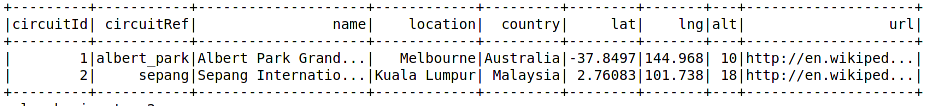
\includegraphics[scale=0.4]{circuits_table.png}
  \centering
  \caption{Tabla circuits}
  \label{fig:circuits}
  \centering
\end{figure}

\begin{figure}
  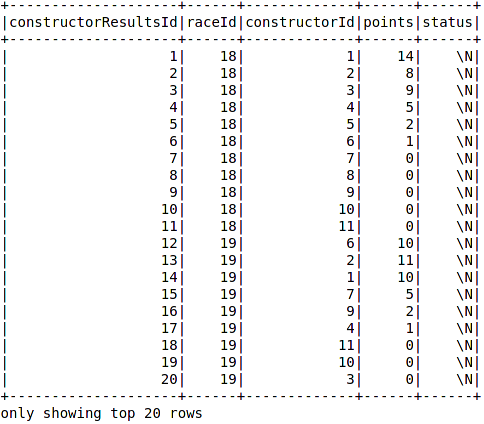
\includegraphics[scale=0.4]{constructor_results_table.png}
  \centering
  \caption{Tabla constructor$\_$results}
  \label{fig:constructorres}
  \centering
\end{figure}

\begin{figure}
  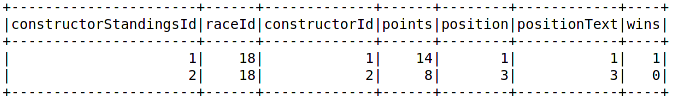
\includegraphics[scale=0.4]{constructor_standings_table.png}
  \centering
  \caption{Tabla constructor$\_$standings}
  \label{fig:constructorstands}
  \centering
\end{figure}

\begin{figure}
  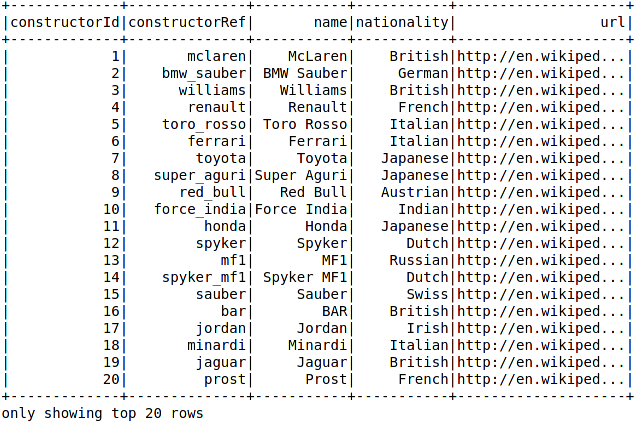
\includegraphics[scale=0.4]{constructors_table.png}
  \centering
  \caption{Tabla constructors}
  \label{fig:constructors}
  \centering
\end{figure}

\begin{figure}
  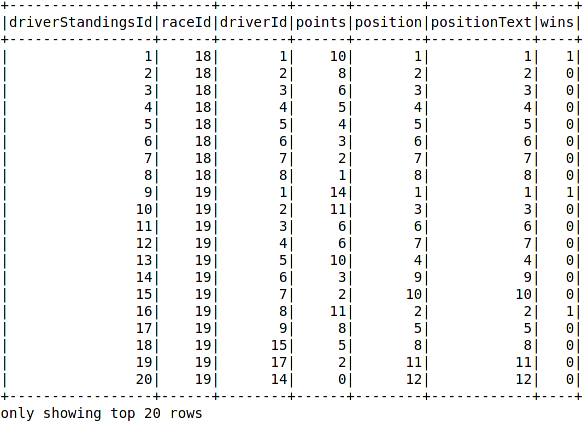
\includegraphics[scale=0.4]{driver_standings_table.png}
  \centering
  \caption{Tabla driver$\_$standings}
  \label{fig:drivstands}
  \centering
\end{figure}

\begin{figure}
  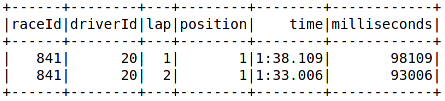
\includegraphics[scale=0.4]{lap_times_table.png}
  \centering
  \caption{Tabla lap$\_$times}
  \label{fig:laptimestab}
  \centering
\end{figure}

\begin{figure}
  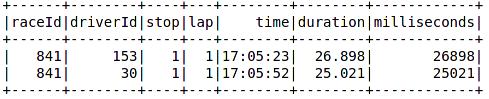
\includegraphics[scale=0.4]{pit_stop_table.png}
  \centering
  \caption{Tabla pit$\_$stops}
  \label{fig:pitstops}
  \centering
\end{figure}

\begin{figure}
  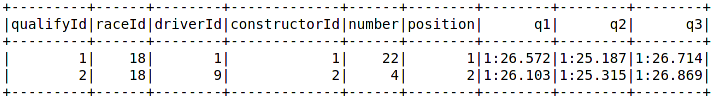
\includegraphics[scale=0.4]{qualifying_table.png}
  \centering
  \caption{Tabla qualifying}
  \label{fig:quali}
  \centering
\end{figure}

\begin{figure}
  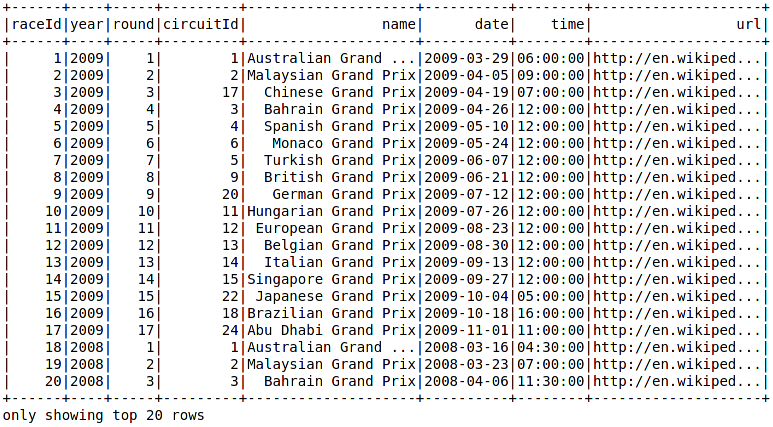
\includegraphics[scale=0.4]{races_table.png}
  \centering
  \caption{Tabla races}
  \label{fig:races}
  \centering
\end{figure}

\begin{figure}
  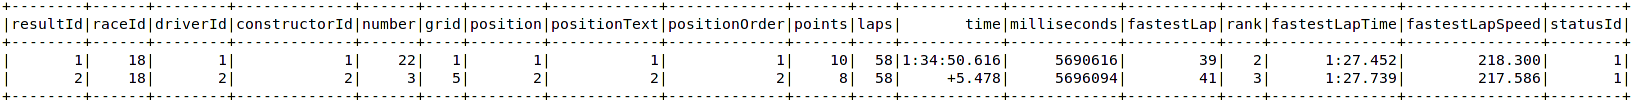
\includegraphics[scale=0.27]{results_table.png}
  \centering
  \caption{Tabla results}
  \label{fig:resultstab}
  \centering
\end{figure}

\begin{figure}
  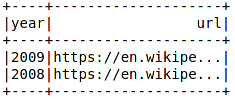
\includegraphics[scale=0.4]{season_table.png}
  \centering
  \caption{Tabla seasons}
  \label{fig:seasonstable}
  \centering
\end{figure}

\begin{figure}
  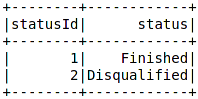
\includegraphics[scale=0.4]{status_table.png}
  \centering
  \caption{Tabla status}
  \label{fig:statustable}
  \centering
\end{figure}

\begin{figure}
  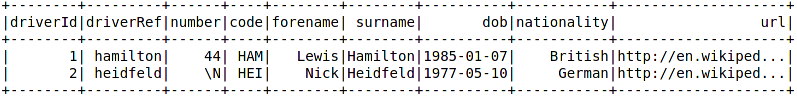
\includegraphics[scale=0.4]{driver_table.png}
  \centering
  \caption{Tabla drivers}
  \label{fig:driverstable}
  \centering
\end{figure}

\subsubsection{Diagrama Entidad-Relación}
\begin{figure}
  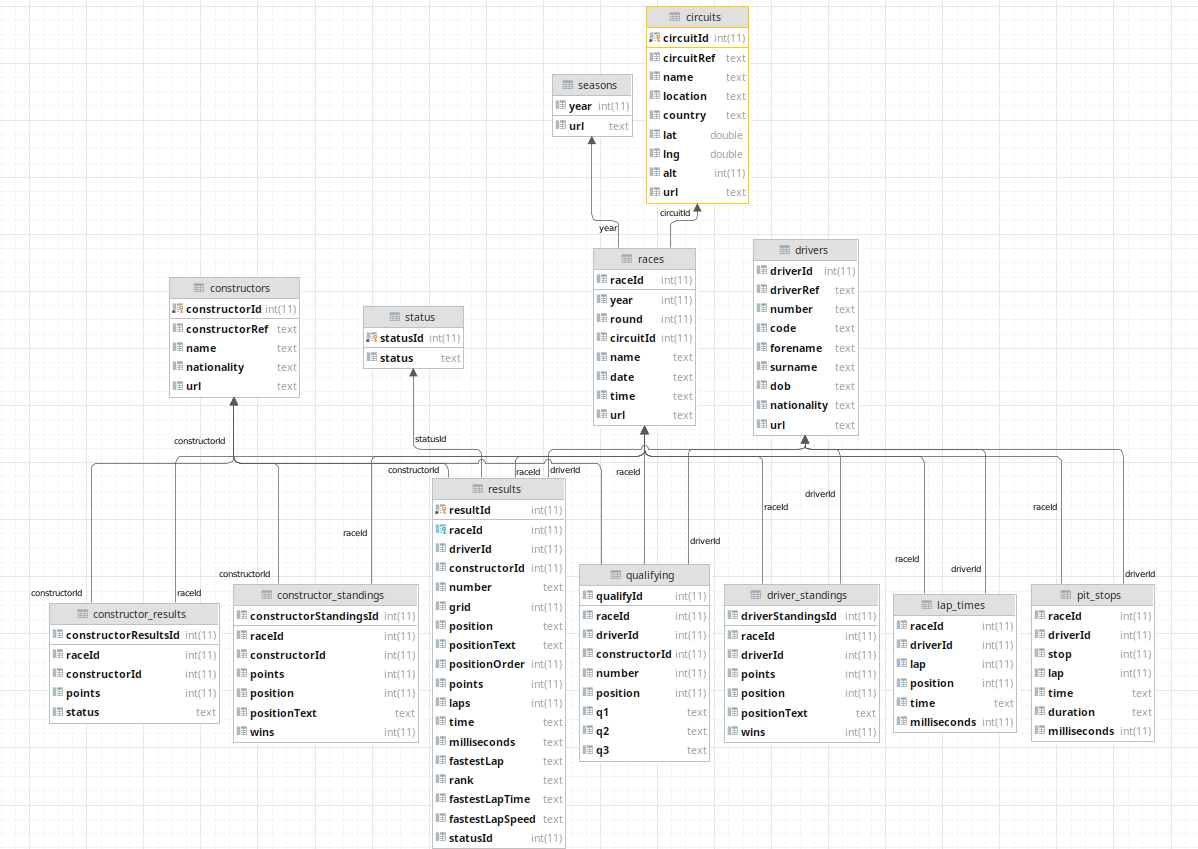
\includegraphics[scale=0.4]{dataset_visualization.png}
  \centering
  \caption{Tabla results}
  \label{fig:datavisualization}
  \centering
\end{figure}



% Fin del documento
\end{document}
